\chapter{Game AI}
%Babbage, Charles -- . . .every game of skill is susceptible of being played by an automaton.
%Minsky, Marvin -- It is not that the games and mathematical problems are chosen because they are clear and simple; rather it is that they give us, for the smallest initial structures, the greatest complexity, so that one can engage some really formidable situations after a relatively minimal diversion into programming. From Semantic Information Processing, p. 12. Cambridge, MA: MIT Press (1968).
% If you'd like to know, I can tell you that in your universe you move freely in three dimensions that you call space. You move in a straight line in a fourth, which you call time, and stay rooted to one place in a fifth, which is the first fundamental of probability. After that it gets a bit complicated, and there's all sort of stuff going on in dimensions thirteen to twenty-two that you really wouldn't want to know about. All you really need to know for the moment is that the universe is a lot more complicated than you might think, even if you start from a position of thinking it's pretty damn complicated in the first place. I can easily not say words like "damn" if it offends you. H2G2

%%% Some characteristics of Game AI
%%% high-level perception, commonsense reasoning, NLP, speech processing,
%%% gesture processing, planning \& counterplanning, cognitive modeling,
%%% plan recognition, soft real-time response, reactive behavior, teamwork,
%%% scheduling, path planning, spatial reasoning, temporal reasoning,
%%% opponent modeling, learning, knowledge acquisition

\begin{verse}\textit{
\\
David: What is the primary goal?\\
Joshua: You should know, Professor. You programmed me.\\
David: Oh, come on. What is the primary goal?\\
Joshua: To win the game.\\
} Wargames (1983)\end{verse}
%\lettrine[image=true, lines=3, findent=3pt, nindent=0pt]{lettrines/O.png}{r}
\lettrine{O}{r}
 is it? ``Game AI'', simultaneously a research topic, an industry standard practice, from a staple to a part of the gameplay. Its uses range from character animation, to behavior modeling and strategic play. In this chapter, we will give our educated guess about the goals of game AI, and review what exists for a broad category of games: single player games, abstract strategy games, partial information and/or stochastic games, computer games. Let us then focus on game-play (from a player point of view) characteristics of theses games so that we can enumerate game AI needs. %%% XXX
%\lettrine[image=true, lines=3, findent=3pt, nindent=0pt]{lettrines/W.png}{hat} is game AI? What are the goals of AI in games? What are its characteristics? Why is game AI an interesting subject for research? 

%%%%%%%%%%%%%%%%%%%%%%%%%%%%%%%%%%%%%%%%%%%%%%%%%%%%%%%%%%%%%%%%%% 

\section{Goals of Game AI}
%\lettrine[lines=1, lhang=.3]{W}{hat} are the goals of game AI?
Non-playing characters (NPC, also called ``mobs'') are here to stay. Being it in ever more immersive single player adventures (The Elder Scrolls V: Skyrim), part of a cooperative gameplay (World of Warcraft, Left 4 Dead) or as helpers on our side or trainers against us (``pets'', strategy games), they are of interest for the game industry, but also for robotics, to study human cognition and for artificial intelligence in the large.

\subsection{Win}
%%%Not solved: humans are the best
During the last decade, the video games industry has seen the emergence of ``e-sport''. It is the professionalization of specific competitive games at the higher levels, as in sports: with spectators, leagues, sponsors, fans and broadcasts. A %non-exhaustive 
list of major electronic sports games includes (but is not limited to): StarCraft: Brood War, Counter-Strike, Quake III, Warcraft III, Halo, StarCraft II. The first game to have had progamers was StarCraft: Brood War, in Korea, with top players earning more than top soccer players. Top players earn more than \$400,000 a year but the professional average is below, around \$50-60,000 a year \citep{TeamLiquidPGMIncome}, against the average South Korean salary at \$16,300 in 2010. Currently, Brood War is being slowly phased out to StarCraft II (still 4.9 millions players in South Korea in 2011 \citep{CitationNeeded}). There are TV channels broadcasting Brood War (OnGameNet, previously also MBC Game) or StarCraft II (GOM TV, streaming) and for which it constitutes a major chunk of the air time. %in 2010 in South Korea, the average salary for a professional StarCraft player was \$60,000 against the average salary at \$16,300\citep{StarCraftPGM}). 
``E-sport'' is important to the subject of game AI because it ensures competitiveness of the human players. It is less challenging to write a competitive AI for game played by few and without competitions than to write an AI for Chess, Go or StarCraft. E-sport, through the distribution of ``replays'' also ensures a constant and heavy flow of human player data to mine and learn from. Finally, cognitive science researchers (like the Simon Fraser University Cognitive Science Lab) study the cognitive aspects (attention, learning, re) of high level RTS playing\citep{CitationNeeded}.

Good human players, through their ability to learn and adapt, and through high-level strategic reasoning, are still undefeated. Single players are often frustrated by the NPC behaviors in non-linear (not fully scripted) games. Nowadays, video games AI could be used part of the gameplay as a challenge to the player. 
This is not the case in most of the games though, in decreasing order of resolution of the problem\footnote{We deal in gameplay potentials here, particularly considering non-linear games, current RPG and MMORPG are often linearly limited \textit{because} of the untracted``world interacting NPC'' AI problem. Otherwise, linear RPG AI fare often better than team FPS AI.}: fast FPS (first person shooters)\newglossaryentry{FPS}{name=FPS,description={First Person Shooter: egocentric shooter game, strong sub-genres are fast FPS, also called ``Quake-likes'', e.g. Quake III; and team/tactical FPS, e.g. Counter-Strike, Team Fortress 2}}, team FPS, RPG (role playing games)\newglossaryentry{RPG}{name=RPG,description={Role Playing Game, e.g. Dungeons \& Dragons based Baldur's Gate}}, MMORPG (Massively Multi-player Online RPG)\newglossaryentry{MMORPG}{name=MMORPG,description={Massively Multi-player Online Role Playing Game, distinct of RPG by the scale of cooperation sometimes needed to achieve a common goal, e.g. Dark Age of Camelot, World of Warcraft}}, RTS (Real-Time Strategy)\newglossaryentry{RTS}{name=RTS,description={Real-Time Strategy games are (mainly) allocentric economic and military simulations from an operational tactical/strategist commander viewpoint, e.g. Command \& Conquer, Age of Empires, StarCraft, Total Annihilation}}. These games in which artificial intelligences do not beat top human players on equal footing requires increasingly more cheats to even be a challenge (not for long as they mostly do not adapt). AI cheats encompass (but are not limited to):
\begin{itemize}
\item RPG NPC often have at least 10 times more hit points (health points) than their human counterparts in equal numbers,
\item FPS bots can see through walls and use perfect aiming,
\item RTS bots see through the ``fog of war'' and have free additional resources.
\end{itemize}
How do we build game robotic players (``bots'', AI, NPC) which can provide some challenge, or be helpful without being frustrating, while staying fun?


\subsection{Fun}
%%%Not solved: humans are the most fun to play with
The main purpose of gaming is entertainment. Of course, there are subgenres of serious gaming or ``gamification'' of learning, but the majority of people playing games are having fun. Cheating AI are not fun, and so the re-playability of single player games is very low. The vast majority of games which are still played after the single player mode are multi-player games, because humans are the most fun to play with. So how do we get game AI to be fun to play with? The answer seems to be 3-fold:
\begin{itemize}
\item For competitive and PvP\newglossaryentry{PvP}{name=PvP,description={Players versus Players}}
(players versus players) games: improve game AI so that it can play well \textit{on equal footing with humans},
\item for cooperative and PvE\newglossaryentry{PvE}{name=PvE,description={Players vs Environment}}
(players vs environment) games: optimize the AI for fun, ``epic wins'': the empowerment of playing your best and just barely winning,
\item give the AI all the tools to adapt the game to the players: game directors (Left 4 Dead, Dark Spore), procedural content generation (Mario PCG).
\end{itemize}
In all cases, a good AI should be able to learn for the players' actions, recognize their behavior to deal with it in the most entertaining way. Examples for a few mainstream games: World of Warcraft instances or StarCraft II missions could be less predictable (less scripted) and always ``just hard enough'', Battlefield 3 or Call of Duty opponents could have a longer life expectancy (5 seconds in some cases), Skyrim's follower NPC could avoid blocking the player in doors, or going in front when she casts fireballs.

\subsection{Programming}
How do game developers want to deal with game AI programming? We have to understand the needs of industry game AI programmers: 
\begin{itemize}
    \item computational efficiency (particularly for real-time games with advanced graphics, the AI CPU budget is low),
    \item game designers often want to remain in control of the behaviors (and editing tools have to be usable by them),
    \item scalability (as much autonomy as possible), ``debugability'' (huge states spaces due to the presence of the player(s)), re-use accross games (game independant logic).
\end{itemize}
So, programmers can ``hard code'' the behaviors and their switches, for some structuring they have finite state machines \citep{FSM_AIGameProgWisdom2003}. This solution does not scale well (exponential increase in the number of transitions), nor do they generate autonomous behavior, and they can be cumbersome for the game designers to interact with. Hierarchical FSM \citep{CitationNeeded} is a partial answer to these problems: they scale better due to the sharing of transitions between macro-states and are more readable for game designers who can zoom-in on macro/englobing states. They still represent way too much programming work for complex behavior and are not more autonomous than classic FSM. Planning (using a search heuristic in the states space) efficiently gives autonomy to virtual characters. Planners like hierarchical task networks (HTN \citep{Erol_htnplanning}, Armed Assault, Killzone 2 \citep{ArmA1_HTN,Killzone2_HTN}) or STRIPS (\citep{FikesSTRIPS}, F.E.A.R \citep{orkinGDC_FEAR}) generate complex behaviors in the space of the combinations of specified states, and the logic can be re-used accross games. The drawbacks can be a large computational budget (for many agents and/or a complex world), the difficulty to specify reactive behavior, and less (or harder) control from the game designers. Behavior trees (Halo 2 \citep{Isla}, Spore) are a popular in-between HTN and HFSM technique providing scability through a tree-like hierarchy, control through tree editing and some autonomy through a search heuristic (for valid nodes).
A transversal technique for ease of use is to program game AI with a script (LUA, Python) or domain specific language (DSL\newglossaryentry{DSL}{name=DSL,description={Domain Specific Language}}). From a programming or design point of view, it will have the drawbacks of the models it is based on. If everything is allowed (low-level inputs and outputs directly in the DSL), everything is possible at the cost of cumbersome programming, debugging and few re-use.

Even with scalable\footnote{both computationally and in the number of lines of codes to write to produce a new behavior} architectures like behavior trees or the autonomy that planning provides, there are limitations (burdens on programmers/designers or CPU/GPU):
\begin{itemize}
    \item complex worlds require either very long description of the state (in propositional logic) or high expressivity (higher order logics) to specify well-defined behaviors,
    \item the search space of possible actions increases exponentially with the interactivity (complexity) of the world, thus requiring ever more efficient pruning techniques,
    \item once human players are in the loop (ain't that the purpose of a game?), uncertainty has to be taken into account. Previous approaches can be ``patched'' to deal with uncertainty, at what cost?
\end{itemize}
Our thesis is that we can learn complex behaviors from exploration or observations (of human players) without the need to be explicitely programmed. Furthermore, the game designers can stay in control by choosing which demonstration to learn from and tuning parameters by hand if wanted. \citet{lehy04} showed it in the case of FPS AI (Unreal Tournament), with \textit{inverse programming} to learn reactive behaviors from human demonstration. We extend it to tactical and even strategic behaviors.

%%%%%%%%%%%%%%%%%%%%%%%%%%%%%%%%%%%%%%%%%%%%%%%%%%%%%%%%%%%%%%%%%% 

\section{Single Player Games}

Single player games are not the main focus of our thesis, but they present a few interesting AI characteristics. They encompass all kinds of human cognitive abilities, from reflexes to higher level thinking.

\subsection{Action games}
%%% Mario, racing, PacMan
Platform games (Mario, Sonic), time attack racing games (TrackMania), solo shoot-them-up (``schmups'', Space Invaders, DodonPachi), sports games and rhythm games (Dance Dance Revolution, Guitar Hero) are games of reflexes, skill and level knowledge. The main components of game AI in these genres is a quick path search heuristic, often with a dynamic environment. There have been Mario \citep{TogeliusMario10}, PacMan \citep{PacManCEC11} and racing competitions \citep{CarRacingWCCI08}. The winners often use (clever) heuristics coupled with a search algorithm (A* for instance). As there are no human opponents, reinforcement learning and genetic programming works well too.

XXX

\subsection{Puzzles}
%%% Myst, Tetris, point and clicks, Patience
Point and click (Monkey Island, Kyrandia, Day of the Tentacle), graphic adventure (Myst, Heavy Rain), (tile) puzzles (Minesweeper, Tetris) games are games of logical thinking and puzzle solving. The main components of game AI in these genres is an inference engine with sufficient domain knowledge (an ontology). AI research is not particularly active in the genre of puzzle games, perhaps because solving them has more to do with writing down the ontology than with using new AI techniques. A classic well-studied logic-based, combinatorial puzzle is Sudoku, which has been formulated as a SAT-solving \citep{lynce2006sudoku} and constraint satisfaction problem \citep{Simonis2005}.

%%%%%%%%%%%%%%%%%%%%%%%%%%%%%%%%%%%%%%%%%%%%%%%%%%%%%%%%%%%%%%%%%% 

\section{Abstract Strategy Games}
%%% http://en.wikipedia.org/wiki/Game_complexity
%%% http://en.wikipedia.org/wiki/Solved_board_games
\subsection{Tic-tac-toe, Minimax}
Tic-tac-toe (noughts and crosses) is a solved game\newglossaryentry{solvedgame}{name={solved game},description={a game whose outcome can be correctly predicted from any position when each side plays optimally}}, meaning that it can be played optimally from each possible position. How did it came to get solved? Each and every possible positions (26,830) have been analyzed by a Minimax (or its variant Negamax) algorithm. Minimax is an algorithm which can be used to determine the optimal score a player can get for a move in a zero-sum game\newglossaryentry{zerosumgame}{name={zero-sum game},description={a game in which the total score of each players, from one player's point-of-view, for every possible strategies, adds up to zero; \textit{i.e.} ``a player benefits only at the expense of others''}}. The Minimax theorem states:
\begin{mythm}
For every two-person, zero-sum game with finitely many strategies, there exists a value V and a mixed strategy for each player, such that (a) Given player 2's strategy, the best payoff possible for player 1 is V, and (b) Given player 1's strategy, the best payoff possible for player 2 is -V.
\end{mythm}
Applying this theorem to Tic-tac-toe, we can say that winning is +1 point for the player and losing is -1, while draw is 0. The exhaustive search algorithm which takes this property into account in described in Algorithm~\ref{alg:minimax}. The result of applying this algorithm to the Tic-tac-toe situation of Fig.~\ref{fig:TTT} is exhaustively represented in Fig.~\ref{fig:minimaxTTT}. For zero-sum games (``strictly competitive games'' as abstract strategy games discussed here), there is a (simpler) Minimax variant called Negamax, shown in Algorithm~\ref{alg:negamax} in Appendix~\ref{apdx:gameAI}.
\begin{algorithm}
\caption{Minimax algorithm}
\label{alg:minimax}
\begin{algorithmic}
\Function{mini}{depth}
    \If{$depth \leq 0$}
        \State \Return $-value()$
    \EndIf
    \State $min \gets +\infty$
    \ForAll{possible moves}
        \State $score \gets maxi(depth-1)$
        \If{$score < min$}
            \State $min \gets score$
        \EndIf 
    \EndFor
    \State \Return $min$
\EndFunction

\Function{maxi}{depth}
    \If{$depth \leq 0$}
        \State \Return $value()$
    \EndIf
    \State $max \gets -\infty$
    \ForAll{possible moves}
        \State $score \gets mini(depth-1)$
        \If{$score > min$}
            \State $max \gets score$
        \EndIf
    \EndFor 
    \State \Return $max$
\EndFunction
\end{algorithmic}
\end{algorithm}

\begin{figure}
\begin{center}
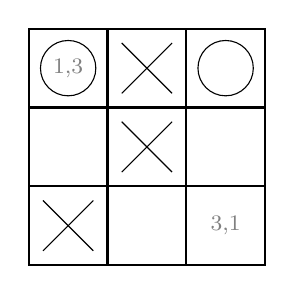
\begin{tikzpicture}
[thick]
  \foreach \x in {1,2,3}
    \foreach \y in {1,2,3}
    {
      \draw (\x,\y) +(-.5,-.5) rectangle ++(.5,.5);
    }

  \draw (1,3) node{\begin{footnotesize}\textcolor{black!50}{1,3}\end{footnotesize}};
  \draw (3,1) node{\begin{footnotesize}\textcolor{black!50}{3,1}\end{footnotesize}};

  \draw (2,3) node{\tikz \draw (-.32,-.32) -- (.32,.32);};
  \draw (2,3) node{\tikz \draw (-.32,.32) -- (.32,-.32);};

  \draw (2,2) node{\tikz \draw (-.32,-.32) -- (.32,.32);};
  \draw (2,2) node{\tikz \draw (-.32,.32) -- (.32,-.32);};

  \draw (1,1) node{\tikz \draw (-.32,-.32) -- (.32,.32);};
  \draw (1,1) node{\tikz \draw (-.32,.32) -- (.32,-.32);};

  \draw (1,3) node{\tikz \draw (0,0) circle (10pt);};

  \draw (3,3) node{\tikz \draw (0,0) circle (10pt);};
\end{tikzpicture}
\caption{A Tic-tac-toe board position, ``circles'' turn to play. The couples of numbers explain the numbering (left to right, bottom to top, starting at 1) of the grid.}
\label{fig:TTT}
\end{center}
\end{figure}

\begin{figure}
%%%\hspace{-0.8cm}
\begin{center}
\begin{tikzpicture}
    [thick,
level 1/.style={sibling distance=42mm},
level 2/.style={sibling distance=14mm},
level 3/.style={sibling distance=7mm}
]
\begin{footnotesize}
  \node[ellipse,draw] {Fig.~\ref{fig:TTT} state}
    child {node[rectangle,draw] {0}
      child {node[circle,draw] {-1}
          edge from parent node[pos=0.5,fill=black!20] {2,1}
        }
      child {node[circle,draw] {0}
          child {node[rectangle,draw] {0}
              child {node[circle,draw] {0}
                edge from parent node[pos=0.5,fill=black!20] {3,2}}
              edge from parent node[pos=0.5,left,fill=black!20] {2,1}
            }
          child {node[rectangle,draw] {0}
              child {node[circle,draw] {-1}
                edge from parent node[pos=0.5,fill=black!20] {2,1}}
              edge from parent node[pos=0.5,fill=black!20] {3,2}
            }
          edge from parent node[pos=0.5,fill=black!20] {3,1}
        }
      child {node[circle,draw] {0}
          child {node[rectangle,draw] {0}
              child {node[circle,draw] {0}
                edge from parent node[pos=0.5,fill=black!20] {3,1}}
              edge from parent node[pos=0.5,left,fill=black!20] {2,1}
            }
          child {node[rectangle,draw] {0}
              child {node[circle,draw] {-1}
                edge from parent node[pos=0.5,fill=black!20] {2,1}}
              edge from parent node[pos=0.5,fill=black!20] {3,1}
            }
          edge from parent node[pos=0.5,fill=black!20] {3,2}
        }
      edge from parent node[pos=0.5,fill=black!20] {1,2}
    }
    child {node[rectangle,draw] {0}
      child {node[circle,draw] {0}
          child {node[rectangle,draw] {0}
              child {node[circle,draw] {-1}
                edge from parent node[pos=0.5,fill=black!20] {3,2}}
              edge from parent node[pos=0.5,left,fill=black!20] {3,1}
            }
          child {node[rectangle,draw] {0}
              child {node[circle,draw] {0}
                edge from parent node[pos=0.5,fill=black!20] {3,1}}
              edge from parent node[pos=0.5,fill=black!20] {3,2}
            }
          edge from parent node[pos=0.5,fill=black!20] {1,2}
        }
      child {node[circle,draw] {0}
          child {node[rectangle,draw] {0}
              child {node[circle,draw] {0}
                edge from parent node[pos=0.5,fill=black!20] {3,2}}
              edge from parent node[pos=0.5,left,fill=black!20] {1,2}
            }
          child {node[rectangle,draw] {0}
              child {node[circle,draw] {0}
                edge from parent node[pos=0.5,fill=black!20] {1,2}}
              edge from parent node[pos=0.5,fill=black!20] {3,2}
            }
          edge from parent node[pos=0.5,fill=black!20] {3,1}
        }
      child {node[circle,draw] {0}
          child {node[rectangle,draw] {0}
              child {node[circle,draw] {-1}
                edge from parent node[pos=0.5,fill=black!20] {3,1}}
              edge from parent node[pos=0.5,left,fill=black!20] {1,2}
            }
          child {node[rectangle,draw] {0}
              child {node[circle,draw] {0}
                edge from parent node[pos=0.5,fill=black!20] {1,2}}
              edge from parent node[pos=0.5,fill=black!20] {3,1}
            }
          edge from parent node[pos=0.5,fill=black!20] {3,2}
        }
      edge from parent node[pos=0.5,fill=black!20] {2,1}
    }
    child {node[rectangle,draw] {0}
      child {node[circle,draw] {0}
          child {node[rectangle,draw] {0}
              child {node[circle,draw] {-1}
                edge from parent node[pos=0.5,fill=black!20] {3,2}}
              edge from parent node[pos=0.5,left,fill=black!20] {2,1}
            }
          child {node[rectangle,draw] {1}
              edge from parent node[pos=0.5,fill=black!20] {3,2}
            }
          edge from parent node[pos=0.5,fill=black!20] {1,2}
        }
      child {node[circle,draw] {-1}
          edge from parent node[pos=0.5,fill=black!20] {2,1}
        }
      child {node[circle,draw] {0}
          child {node[rectangle,draw] {0}
              child {node[circle,draw] {-1}
                edge from parent node[pos=0.5,fill=black!20] {2,1}}
              edge from parent node[pos=0.5,left,fill=black!20] {1,2}
            }
          child {node[rectangle,draw] {0}
              child {node[circle,draw] {-1}
                edge from parent node[pos=0.5,fill=black!20] {1,2}}
              edge from parent node[pos=0.5,fill=black!20] {2,1}
            }
          edge from parent node[pos=0.5,fill=black!20] {3,2}
        }
      edge from parent node[pos=0.5,fill=black!20] {3,1}
    }
    child {node[rectangle,draw] {0}
      child {node[circle,draw] {0}
          child {node[rectangle,draw] {0}
              child {node[circle,draw] {0}
                edge from parent node[pos=0.5,fill=black!20] {3,1}}
              edge from parent node[pos=0.5,left,fill=black!20] {2,1}
            }
          child {node[rectangle,draw] {1}
              edge from parent node[pos=0.5,fill=black!20] {3,1}
            }
          edge from parent node[pos=0.5,fill=black!20] {1,2}
        }
      child {node[circle,draw] {-1}
          edge from parent node[pos=0.5,fill=black!20] {2,1}
        }
      child {node[circle,draw] {0}
          child {node[rectangle,draw] {0}
              child {node[circle,draw] {-1}
                edge from parent node[pos=0.5,fill=black!20] {2,1}}
              edge from parent node[pos=0.5,left,fill=black!20] {1,2}
            }
          child {node[rectangle,draw] {0}
              child {node[circle,draw] {0}
                edge from parent node[pos=0.5,fill=black!20] {1,2}}
              edge from parent node[pos=0.5,fill=black!20] {2,1}
            }
          edge from parent node[pos=0.5,fill=black!20] {3,1}
        }
      edge from parent node[pos=0.5,fill=black!20] {3,2}
    };
\end{footnotesize}
\end{tikzpicture}
\end{center}
\caption{Minimax tree with initial position at Fig.~\ref{fig:TTT} state, \textbf{nodes} are states and \textbf{edges} are transitions, labeled with the move. Leafs are end-game states: 1 point for the win and -1 for the loss. Player is ``circles'' and plays first (first edges are player's moves).}
\label{fig:minimaxTTT}
\end{figure}
\subsection{Checkers, Alpha-beta}
Checkers, Chess and Go are also zero sum, perfect-information\newglossaryentry{perfectinformationgame}{name={perfect-information game},description={a game in which all the players have complete knowledge of the (board) state of the game}}, partisan\newglossaryentry{partisangame}{name={partisan game},description={a game which is not impartial, in which a player can do actions another can not do (move a faction while the other player(s) cannot)}}, deterministic strategy game. Technically, they all can be solved by exhaustive Minimax. In practice though, it is often intractable: their bounded versions are at least in \textsc{pspace} and their unbounded versions are \textsc{exptime}-hard \citep{GPC}. The state space complexity of Checkers is the smallest of the 3 above-mentioned games with $\approxeq 5.10^20$ possible positions, and as a matter of fact, Checkers have been solved completely\citep{SchaefferBBKMLLS07}. We can see the complexity of Minimax as $O(b^d)$ with $b$ the average branching factor of the tree (to search) and $d$ the average length (depth) of the game. For Checkers $b \approxeq 10$, while the mean game length is 70 \citep{allis1994}. It is already too large to have been solved by Minimax alone (on current hardware). From 1989 to 2007, there were artificial intelligences competitions on Checkers, all using at least alpha-beta pruning: a technique to make efficient cuts in the Minimax search tree while not losing optimality.

Alpha-beta pruning (see Algorithm~\ref{alg:alphabeta}) is a branch-and-bound algorithm which (if the best nodes are searched first) can reduce Minimax to a $O(b^{d/2})=O(\sqrt{b^d})$ complexity ($O(b^{3d/4})$ for a random ordering of nodes). $\alpha$ is the maximum score than we (the maximizing player) are assured to get given what we already evaluated, while $\beta$ is the minimum score than the minimizing player is assured to get. When evaluating more and more nodes, we can only get a better estimate and so $\alpha$ can only increase while $\beta$ can only decrease. %If we find a node for us with an expected value below $\alpha$, we do not have to consider its subtree because it's sub-optimal play. If we find an expected value above $\beta$, it's sub-optimal play for the opponent. 
\begin{algorithm}
\caption{Alpha-beta algorithm}
\label{alg:alphabeta}
\begin{algorithmic}
\Function{alphabeta}{node,depth,$\alpha$,$\beta$,player}
    \If{$depth \leq 0$}
        \State \Return $value(player)$
    \EndIf
    \If{$player == us$}
        \ForAll{possible moves}
            \State $\alpha \gets \max{(\alpha, alphabeta(child,depth-1,\alpha,\beta,opponent))}$
            \If{$\beta \leq \alpha$}
                \State \textbf{break}
            \EndIf
        \EndFor
        \State \Return $\alpha$
    \Else
        \ForAll{possible moves}
            \State $\beta \gets \min{(\beta, alphabeta(child,depth-1,\alpha,\beta,us))}$
            \If{$\beta \leq \alpha$}
                \State \textbf{break}
            \EndIf
        \EndFor
        \State \Return $\beta$
    \EndIf
\EndFunction
\end{algorithmic}
\end{algorithm}
If we find a node for which $\beta$ becomes less than $\alpha$, it means that this position results from sub-optimal play. When it is because of an update of $\beta$, the sub-optimal play is on the side of the maximizing player (his $\alpha$ is not high enough to be optimal and/or the minimizing player has a winning move faster in the current sub-tree) and this situation is called an $\alpha$ cut-off. On the contrary, when the cut results from an update of $\alpha$, it is called a $\beta$ cut-off and means that the minimizing player would have to play sub-optimally to get into this sub-tree. When Starting the game, $\alpha$ is initialized to $-\infty$ and $\beta$ to $+\infty$. A worked example is given on Figure~\ref{fig:alphabeta}.
\tikzset{
alphacut/.style={postaction={decorate},
        decoration={markings,mark=at position .50 with {\draw (0.05,-.28)--(0.05,.28);\draw (-.05,-.28)--(-.05,.28);\node[right]{$\ \ \alpha \ cut$};}}},
betacut/.style={postaction={decorate},
        decoration={markings,mark=at position .50 with {\draw (0.05,-.28)--(0.05,.28);\draw (-.05,-.28)--(-.05,.28);\node[right]{$\ \ \beta \ cut$};}}},
}
\begin{figure}
%%%\hspace{-0.8cm}
\begin{center}
\begin{tikzpicture}
    [thick,
level 1/.style={sibling distance=32mm},
level 2/.style={sibling distance=14mm},
level 3/.style={sibling distance=7mm}
]
\begin{small}
  \node[circle,draw] (top) {3}
    child {node[rectangle,draw] (a) {3}
        child {node[circle,draw] (d3) {3}
            child {node[rectangle,draw] (d4) {2}}
            child {node[rectangle,draw] {3}}
        }
        child {node[circle,draw] (A) {}
            child {node[rectangle,draw] {5}}
            child {node[rectangle,draw] {} edge from parent[betacut]}
        }
    }
    child {node[rectangle,draw] (b) {0}
        child {node[circle,draw] {0}
            child {node[rectangle,draw] {0}}
        }
        child {node[circle,draw] (B) {}
            child {node[rectangle,draw] {}}
            child {node[rectangle,draw] {}}
            edge from parent[alphacut]
        }
    }
    child {node[rectangle,draw] (c) {2}
        child {node[circle,draw] {2}
            child {node[rectangle,draw] {2}}
            child {node[rectangle,draw] {1}}
        }
        child {node[circle,draw] {}
            child {node[rectangle,draw] {}}
            child {node[rectangle,draw] {}}
            edge from parent[alphacut]
        }
    };
    \node [blue,left] at (top.west) (d1) {$\alpha = 3$};
    \node [blue,left] at (a.west) (d2) {$\beta = 3$};
    \node [blue,left] at (b.west) {$\beta = 0$};
    \node [blue,left] at (c.west) {$\beta = 2$};
    \node [right] at (A.east) {$A$};
    \node [right] at (b.east) {$B$};
    \node [right] at (c.east) {$C$};
    \node [left,align=flush left] at (d1.west) {\textsc{Max}\ \ \ };
    \node [left,align=flush left] at (d2.west) {\textsc{Min}\ \ \ };
    \node [left] at (d3.west) {\textsc{Max}\ \ \ };
    \node [left] at (d4.west) {\textsc{Min}\ \ \ };
\end{small}
\end{tikzpicture}
\end{center}
\caption{Alpha-beta cuts on a Minimax tree, \textbf{nodes} are states and \textbf{edges} are transitions, labeled with the values of positions at the bottom (max depth). Here is the trace of the algorithm: \textbf{1.} descend leftmost first and evaluated 2 and 3, \textbf{2.} percolate max(2,3) higher up to set $\beta = 3$, \textbf{3.} $\beta$-cut in $A$ because its value is at least 5 (which is superior to $\beta=3$), \textbf{4.} Update of $\alpha=3$ at the top node, \textbf{5.} $\alpha$-cut in $B$ because it is at most 0 (which is inferior to $\alpha=3$), \textbf{6.} $\alpha$-cut in $C$ because it is at most 2, \textbf{7.} conclude the best value for the top node is 3.}
\label{fig:alphabeta}
\end{figure}
Prior to Checkers being solved (meaning that we have a database of which moves to play for all positions resulting from optimal play), or if playing against a sub-optimal opponent, Alpha-beta is going to be helpful to search much deeper than Minimax in the same allowed time. The best Checkers program (since the 90s), which is also the project which solved Checkers \citep{SchaefferBBKMLLS07}, Chinook, has openings and end-game (for lest than eight pieces of fewer) books, and for the mid-game (when there are more possible moves) relies on a deep search algorithm. So, appart for the beginning and the ending of the game, for which it plays by looking up a database, it used a search algorithm. As Minimax and Alpha-beta are depth first search heuristics, all programs which have to answer in a fixed limit of time use \textit{iterative deepening}, a technique which consists in fixing limited depth which will be considered maximal and evaluating this position. As it does not relies in winning moves at the bottom (remember, the search space is too big in $branching^{depth}$), we need moves evaluation heuristics. We then iterate on growing the maximal depth for which we consider moves, but we are at least sure to have a move to play in a short time (at least the greedy depth 1 found move).

\subsection{Chess, Heuristics}
With a branching factor of $\approxeq 35$ and an average game length of 80 moves \citep{Shannon_1950}, the average game-tree complexity of chess is $35^{80}\approxeq 3.10^{123}$. \citet{Shannon_1950} also estimated the number of possible actions (Shannon number) to be of the order of $10^{43}$. Chess AI needed a little more than just Alpha-beta to win against top human players (not that Checkers could not benefit it!), particularly on 1996 hardware (first win of a computer against a reigning world champion, Deep Blue on Garry Kasparov). Once an AI has openings and ending books (databases to look-up for classical moves), how can we search deeper during the game, or how can we evaluate better a situation? In iterative deepening Alpha-beta (or other search algorithms like Negascout or MTD-f), one needs to know the value of a move at the maximal depth. If it does not correspond to the end of the game, there is a need for a evaluation heuristic. Some may be straight forward, like the resulting value of an exchange in pieces points. But some strategies sacrifice a queen in favor of a more avantageous tactical position or a checkmate, so evaluation heuristics need to take tactical positions into account. In Deep Blue, the evaluation function had 8000 cases, with 4000 positions in the openings book, all learned from 700,000 grandmaster games \citep{DeepBlue}. Nowadays, Chess programs are better than deep blue and generally also search less positions. For instance, Pocket Fritz (HIARCS engine) beats current grandmasters \citep{CitationNeeded} while evaluating 20,000 positions per second (740 MIPS on a smartphone) against Deep Blue's (11.38 GFlops) 200 millions per second.

\subsection{Go, Monte-Carlo Tree Search}
With an estimated number of legal 19x19 Go positions of $2.081681994 * 10^{170}$ \cite{tromp2006}, and an average branching factor above Chess for gobans above 9x9, Go sets another limit for AI. MoGo \citep{GellyUCT, Gelly2006} introduced Upper Confidence Bounds for Trees (UCT\newglossaryentry{UCT}{name=UCT,description={Upper Confidence Bounds for Trees}}) for Monte-Carlo Tree Search (MCTS\newglossaryentry{MCTS}{name=MCTS,description={Monte-Carlo Tree Search}}) in Go AI successfully (being the best 9x9 and 13x13 Go program and the first to win against a pro on 9x9). The approach of MCTS is to randomly sample in the search tree (which is too big to be searched entirely), instead of systematically expanding the build tree as in Minimax. For that, all we need is to have, for each node $node$ in the search tree, $Q(node)$ the sum of the simulations rewards on all the runs through $node$, and $N(node)$ the visits count of $node$. Algorithm~\ref{alg:mcts} details the MCTS algorithm and Fig.~\ref{fig:mcts} explains the principle.
\begin{algorithm}
\caption{Monte-Carlo Tree Search algorithm. 
\textsc{ExpandFrom}$(node)$ is the tree (growing) policy function on how to select where to search from situation $node$ (exploration or exploitation?) and how to expand the game tree (deep-first, breadth-first, heuristics?) in case of untried actions. \textsc{Evaluate}$(tree)$ may have 2 behaviors: \textbf{1.} if $tree$ is complete (terminal), it gives an evaluation according to games rules, \textbf{2.} if $tree$ is incomplete, it has to give an estimation, either through simulation (for instance play at random) or an heuristic. \textsc{BestChild} picks the action that leads to the better value/reward from $node$. \textsc{Merge}$(node, tree)$ changes the existing tree (with $node$) to take all the $Q(\nu) \forall \nu \in tree$ (new) values into account. If $tree$ contains new nodes (there were some exploration), they are added to $node$ at the right positions.}
\label{alg:mcts}
\begin{algorithmic}
\Function{MCTS}{$node$}
    \While{computational time left}
        \State $tree \gets$ \textsc{ExpandFrom}$(node)$
        \State $tree.values \gets$ \textsc{Evaluate}$(tree)$
        \State \textsc{Merge}$(node, tree)$
    \EndWhile
    \State \Return \textsc{BestChild}$(node)$
\EndFunction
\end{algorithmic}
\end{algorithm}
\begin{algorithm}
\caption{UCB1 \textsc{ExpandFrom}}
\label{alg:expandfrom}
\begin{algorithmic}
\Function{ExpandFrom}{$node$}
    \If{$node$ is terminal}
        \State \Return $node$ \ \ \ \ \texttt{// terminal}
    \EndIf
    \If{$\exists c \in node.children\ s.t.\ N(c)=0 $}
        \State \Return $c$ \ \ \ \ \texttt{// grow}
    \EndIf
    \State \Return \textsc{ExpandFrom}$(\argmax_{c \in node.children)} \frac{Q(c)}{N(c)}+k\sqrt{\frac{\ln N(node)}{N(c)}})$ \ \ \ \ \texttt{// select}
\EndFunction 
\end{algorithmic}
\end{algorithm}

\begin{figure}
\begin{center}
\tikzset{
%/.style={postaction={decorate},
%        decoration={markings,mark=at position .50 with {\draw (0.05,-.28)--(0.05,.28);\draw (-.05,-.28)--(-.05,.28);\node[right]{$\ \ \beta \ cut$};}}},
}
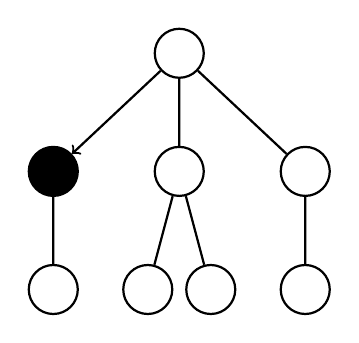
\begin{tikzpicture}
[
thick,
level 1/.style={sibling distance=16mm},
level 2/.style={sibling distance=8mm}
]
\begin{footnotesize}
  \node[circle,draw,inner sep=2.2mm] {}
    child {node[circle,draw,inner sep=2.2mm,fill] {} edge from parent [->]
        child {node[circle,draw,inner sep=2.2mm] {} edge from parent [-]}
        %child {node[circle,draw] {}}
    }
    child {node[circle,draw,inner sep=2.2mm] {}
        child {node[circle,draw,inner sep=2.2mm] {}
        }
        child {node[circle,draw,inner sep=2.2mm] {}
        }
    }
    child {node[circle,draw,inner sep=2.2mm] {}
        child {node[circle,draw,inner sep=2.2mm] {}
        }
    };
\end{footnotesize}
\end{tikzpicture}
\hspace{1cm}
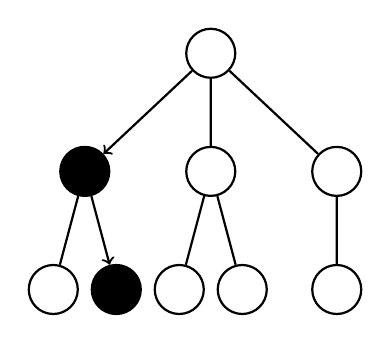
\begin{tikzpicture}
[
thick,
level 1/.style={sibling distance=16mm},
level 2/.style={sibling distance=8mm}
]
\begin{footnotesize}
  \node[circle,draw,inner sep=2.2mm] {}
    child {node[circle,draw,inner sep=2.2mm,fill] {} edge from parent [->]
        child {node[circle,draw,inner sep=2.2mm] {} edge from parent [-]}
        child {node[circle,draw,inner sep=2.2mm,fill] {} edge from parent [->]}
        %child {node[circle,draw,inner sep=2.2mm] {}}
    }
    child {node[circle,draw,inner sep=2.2mm] {}
        child {node[circle,draw,inner sep=2.2mm] {}
        }
        child {node[circle,draw,inner sep=2.2mm] {}
        }
    }
    child {node[circle,draw,inner sep=2.2mm] {}
        child {node[circle,draw,inner sep=2.2mm] {}
        }
    };
\end{footnotesize}
\end{tikzpicture}
\hspace{1cm}
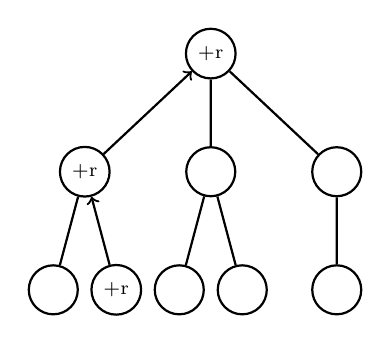
\begin{tikzpicture}
[
thick,
level 1/.style={sibling distance=16mm},
level 2/.style={sibling distance=8mm}
]
\begin{scriptsize}
  \node[circle,draw] {+r}
    child {node[circle,draw] {+r} edge from parent [<-]
        child {node[circle,draw,inner sep=2.2mm] {} edge from parent [-]}
        child {node[circle,draw] {+r} edge from parent [<-]}
        %child {node[circle,draw] {}}
    }
    child {node[circle,draw,inner sep=2.2mm] {}
        child {node[circle,draw,inner sep=2.2mm] {}
        }
        child {node[circle,draw,inner sep=2.2mm] {}
        }
    }
    child {node[circle,draw,inner sep=2.2mm] {}
        child {node[circle,draw,inner sep=2.2mm] {}
        }
    };
\end{scriptsize}
\end{tikzpicture}
\caption{An iteration of the \textbf{while} loop in MCTS, from left to right:
\textsc{ExpandFrom} select, \textsc{ExpandFrom} grow, \textsc{Evaluate} \& \textsc{Merge}.}
\label{fig:MCTS}
\end{center}
\end{figure}

UCT specializes MCTS in that it specifies \textsc{ExpandFrom} (as in Algorithm.~\ref{alg:expandfrom}) tree policy with a specific exploration-exploitation trade-off. UCB1 \citep{BanditBased} views the tree policy as a multi-armed bandit problem and so \textsc{ExpandFrom}$(node)$ UCB1 chooses the arms with the best upper confidence bound: $$\argmax_{c \in node.children} \frac{Q(c)}{N(c)}+k\sqrt{\frac{\ln N(node)}{N(c)}}$$ in which $k$ fixes the exploration-exploitation trade-off: $\frac{Q(c)}{N(c)}$ is simply the average reward when going through $c$ so we have exploitation only for $k=0$ and exploration only for $k=\infty$.

\citet{BanditBased} showed that the probability of selecting sub-optimal actions converges to zero and so that UCT MCTS converges to the minimax tree and so is optimal. Empirically, they found several convergences rates of UCT to be in $O(b^{d/2})$, as fast as Alpha-beta tree search, and able to deal with larger problems (with some error). For a broader survey on MCTS methods, see \citep{MCTSsurvey}.

With Go, we see clearly that humans do not play the game using the same approach. Top Go players can reason about their opponent's move, but they seem to be able to do it in a qualitative manner, at another scale. So, while tree search algorithms help a lot for tactical play in Go, particularly by integrating openings/ending knowledge, pattern macthing algorithms are not yet at the strategical level of human players. When a MCTS algorithm learns something, it stays at the level of possible actions (even considering positional hashing), while the human player seems to be able to generalize, and re-use heuristics learned at another level.

%%%%%%%%%%%%%%%%%%%%%%%%%%%%%%%%%%%%%%%%%%%%%%%%%%%%%%%%%%%%%%%%%% 

\section{Games with Uncertainty}
An exhaustive list of games or even of games genres is beyond the scope/range (XXX) of this thesis. %On the other hand, we will explain games for which randomness or incomplete information plays a key role with not-so-basic examples. 
All uncertainty boils down to incompleteness of information, being it the physics of the dice being thrown or the inability to measure what is happening in the opponent's brain. However,  we will speak of 2 types (sources) of uncertainty: extensional uncertainty, which is due to incompleteness in direct, measurable information, and intentional uncertainty, which is related to randomness in the game or in (the opponent's) decisions. The purest extensional uncertainty being acting without sensing while the purest intentional uncertainty would be for our acts to be the result of a perfect random generator. The uncertainty coming from the opponent's mind/cognition lies in between, depending on the simplicity to model the game as an optimization procedure. The harder the game is to model, the harder it is to model the trains of thoughts our opponents can follow.

\subsection{Monopoly}
In Monopoly, there is few hidden information (\textit{Chance} and \textit{Community Chest} cards only), but there is randomness in the throwing of dice\footnote{Note that the sum of two uniform distributions is not a uniform but a Irwin-Hall, $\forall n>1, P([\sum_{i=1}^n{(X_i\in U(0,1))}]=x) \propto \frac{1}{(n-1)!}\sum_{k=0}^n(-1)^k{n\choose k}\max{((x-k)^{n-1},0)}$, converging towards a Gaussian (central limit theorem).}, and a substantial influence of skill (player's decision). A very basic playing strategy would be to just look at the ruturn on investment (ROI) with regard to prices, rents and frequencies, choosing only based on the money you have and the possible actions of buying or not. A less naive way to play should evaluate the questions of buying with regard to what we already own, what others own, our cash and advancement in the game. The complete state space is huge (places for each players $\times$ their money $\times$ their possessions), but according to \cite{MonopolyMarkov}, we can model the game for one player (as he has no influence on the dice rolls and decisions of others) as a Markov process on 120 ordered pairs: 40 board spaces $\times$ possible number of doubles rolled so far in this turn (0, 1, 2). With this model, it is possible to compute more than simple ROI and derive applicable and interesting strategies. So, even in monopoly, which is not lottery playing or simple dice throwing, a simple probabilistic modeling yields a robust strategy. Additionally, \cite{MonopolyFrayn05} used genetic algorithms to generate the most efficient strategies for portfolio management. %We observe that the main difficulty of Monopoly: randomness in a gameplay in which we have to make up a strategy, can be dealt with with probabilistic modeling. 

Monopoly is an example of a game in which we have complete direct information about the state of the game, intentional uncertainty due to the roll of the dice (randomness) can be dealt with thanks to probabilistic modeling (Markov processes here). The opponent's actions are relatively easy to model due to the fact that the goal is to maximize cash and that there are not many different efficient strategies (not many Nash equilibrium if it were a stricter game) to attain it. In general, the presence of chance does not invalidates previous (game theoretic / game trees) approaches but transforms exact computational techniques into stochastic ones: finite states machines become probabilistic Bayesian networks for instance.

%\subsection{Diplomacy}
%\subsection{Bridge}
\subsection{Battleship}
Battleship (also called ``naval combat'') is a guessing game generally played with two 10x10 grids for each players: one is the player's ships grid, and one is to remember/infer the opponent's ships positions. The goal is to guess where the enemy ships are and sink them by firing shots (torpedoes). There is \textbf{incompleteness} of information but no randomness. Incompleteness can be dealt with with probabilistic reasoning. The classic setup of the game consist in two ships of length 3 and one ship of each lengths of 2, 4 and 5; in this setup, there are 1,925,751,392 possible arrangements for the ships. The way to take advantage of all possible information is to update the probability that there is a ship for all the squares each time we have additional information. So for the 10x10 grid we have a 10x10 matrix $O_{1:10,1:10}$ with $O_{i,j} \in \{true,false\}$ being the $i$th row and $j$th column random variable of the case being occupied. With $ships$ being unsunk ships, we always have $$\sum_{i,j}P(O_{i,j}=true) = \frac{\sum_{k\in ships}length(k)}{10 \times 10}$$. For instance for a ship of size 3 alone at the beginning we can have prior distributions on $O_{1:10,1:10}$ by looking at combinatorics of its placements (see Fig.~\ref{fig:battleship}). We can also have priors on where the opponent likes to place her ships. Then each round we will either hit or miss in $i,j$. When we hit, we know $P(O_{i,j}=true)=1.0$ and will have to revise the probabilities of surrounding areas, and everywhere if we learned the size of the ship, with possible placement of ships. If we did not sunk a ship, the probabilities of uncertain (not 0.0 or 1.0) positions around $i,j$ will be highered according to the sizes of remaining ships. If we miss, we know $P(O_{i,j})=false$ and can also revise (lower) the surrounding probabilities, an example of that effect is shown in Fig.~\ref{fig:battleship}. 

Battleship is a game with few intensional uncertainty (no randomness), particularly because the goal quite strongly conditions the action (sink ships as fast as possible) but a large part of extensional uncertainty (incompleteness of direct information), which goes down rather quickly once we act, if we update a probabilistic model of the map/grid. If we compare Battleship to a variant in which we could see the adversary board, playing would be straightforward (just hit ships we know the position on the board), now in real Battleship we have to model our uncertainty due to the incompleteness of information, without even beginning to take into account the psychology of the opponent in placement as a prior. The cost of solving an imperfect information game increases greatly from its perfect information variant: it seems to be easier to model stochasticity (chance, a source of randomness) than to model a hidden (complex) system for which we only observe (indirect) effects.

\begin{figure}[h!]
\begin{center}
\includegraphics[width=7.8cm]{images/battleship_board_3_init_annotated.png} \includegraphics[width=7.8cm]{images/battleship_board_3_1miss.png}
\caption{Left: visualization of probabilities for squares to contain a ship of size 3 ($P(O_{i,j})=true$) initially, assuming uniform distribution of this type of ship. Annotations correspond to the \textit{number of combinations} (on six, the maximum number of conformations), Right: same probability after a miss in (5, 5). The larger the white area, the higher the probability.}
\label{fig:battleship}
\end{center}
\end{figure}


\subsection{Poker}
Poker\footnote{We deal mainly with the \textit{Limit Hold'em} variant of Poker.} is a zero-sum (without the house's cut), imperfect information and stochastic betting game. Poker ``AI'' is as old as game theory \citep{nash51a}, but the research effort for human-level Poker AI started in the end of the 90s. The interest for Poker AI is such that there are annual AAAI computer Poker competitions\footnote{\url{http://www.computerpokercompetition.org/}}. \citet{Billings98pokeras} defend Poker as an interesting game for decision-making research, %combining imperfect information with randomness. The
because the task of building a good/high level Poker AI (player) entails to take decisions with incomplete information about the state of the game, incomplete information about the opponents' intentions, and model their thoughts process to be able to bluff efficiently. A Bayesian network can combine these uncertainties and represent the player's hand, the opponents' hands and their playing behavior conditioned upon the hand, as in \citep{Korb99bayesianpoker}. A simple ``risk evaluating'' AI (folding and raising according to the outcomes of its hands) will not prevail against good human players. Bluffing, as described by \citet{VonNeumannMorgenstern1944} ``to create uncertainty in the opponent's mind'', is an element of Poker which needs its own modeling. \citet{Southey05bayesbluff} also give a Bayesian treatment to Poker, separating the uncertainty resulting from the game (draw of cards) and from the opponents' strategies, and focusing on bluff. From a game theoretic point of view, Poker is a \textit{Bayesian game}, which needs extensive form modeling (possible game trees along with the agents' information state). \citet{Koller97representationsand} used the sequence form transformation, the set of realization weights of the sequences of moves, %of extensive form with informations sets,
to search over the space of randomized strategies for Bayesian games automatically. Unfortunately, strict game theoretic optimal strategies for full-scale Poker are not tractable this way, two players Texas Hold'em having a state space $\approxeq O(10^18)$. \citet{BillingsBDHSSS03} approximated the game-theoretic optimal strategies through abstraction and are able to beat strong human players (not world-class opponents).

Poker is a game with both extensional and intentional uncertainty, from the fact that the opponents' hands are hidden, the chance in the draw of the cards, the opponents' model about the game state and their model about our mental state(s) (leading our decision(s)). While the iterated reasoning (``if she does A, I can do B'') is (theoretically) finite in Chess due to perfect information, it is not the case in Poker (``I think she thinks I think...''). The combination of different sources of uncertainty (as in Poker) makes it complex to deal with it (somehow, the sources of uncertainty must be separated), and we will see that both these sources of uncertainties arise (at different levels) in video games.

%%%%%%%%%%%%%%%%%%%%%%%%%%%%%%%%%%%%%%%%%%%%%%%%%%%%%%%%%%%%%%%%%% 

\section{FPS}

\subsection{Gameplay and AI}
First person shooters gameplay consist in controlling an agent in first person view, centered on the weapon, a gun for instance. The firsts FPS popular enough to bring the genre its name were Wolfeinstein 3D and Doom, by iD Software. Other classic FPS (series) include Duke Nukem 3D, Quake, Half-Life, Team Fortress, Counter-Strike, Unreal Tournament, Tribes, Halo, Medal of Honor, Call of Duty, Battlefield, etc. The distinction between ``fast FPS'' (e.g. Quake series, Unreal Tournament series) and others is made on the speed at which the player moves. In ``fast FPS'', the player is always jumping, running much faster and playing more in 3 dimensions than on discretely separate 2D ground planes. Game types include (but are not limited to):
\begin{itemize}
    \item single-player missions, depending of the game design.
    \item capture-the-flag (CTF), in which a player has to take the flag inside the enemy camp and bring it back in her own base.
    \item free-for-all (FFA), in which there are no alliances.
    \item team deathmatch (TD), in which two (or more) teams fight on score.
    \item various gather and escort (including hostage or payload), in which one team has to find and escort something/somebody to another location.
    \item duel/tournament/deathmatch, 1 vs 1 matches (mainly ``fast FPS'').
\end{itemize}
Some games allow for instant (or delayed, but asynchronous to other players) respawn, most likely in the ``fast FPS'' (Quake-like) games, while in others, the player has to wait for the end of the round to respawn. In some games, weapons, ammunitions, health, armor and items can be picked on the ground (mainly ``fast FPS''), in others, they are fixed at the start or can be bought in game (with points). The map design can make the gameplay vary a lot, between indoors, outdoors, arena-like or linear maps. According to maps and gameplay styles, combat may be well-prepared with ambushes, sniping, indirect (zone damages), or close proximity (even to fist weapons). Most often, there are strong tactical positions and effective ways to attack them. While ``skill'' (speed of the movements, accuracy of the shots) is easy to emulate for an AI, team-play is much harder for bots and it is always a key ability. Team-play is the combination of distributed evaluation of the situation, planning and distribution of specialized tasks. Very high skill also requires integrating over enemy's tactical plans and positions to be able to take indirect shots (grenades for instance) or better positioning (coming from their back), which is hard for AI too. An example of that is that very good human players consistently beat the best bots (nearing 100\% accuracy) in Quake III (which is an almost pure skill ``fast FPS''), because they take advantage of being seen just when their weapons reload or come from their back. Finally, bots which equal the humans by a higher accuracy are less fun to play with: it is a frustrating experience to be shot across the map, by a bot which was stuck in the door because it was pushed out of its trail.

\subsubsection{State of the art}

\begin{itemize}
\item Quake 3 AI (industry standard w/o squad AI) \citep{waveren-02-artificial}
\item Killzone 2, F.E.A.R \citep{orkinGDC_FEAR} (planning), Crysis 2, BF3: industry standards with squad AI
\item Research:
\begin{itemize}
\item \citep{lehy04}
\item \citep{Laird01} (cognitive architecture)
\item others (\citep{Hladky_anevaluation} ANN, ...)
\item UT Challenge (c.f. CIG)
\end{itemize}
\end{itemize}
\subsubsection{Challenges}

%%%%%%%%%%%%%%%%%%%%%%%%%%%%%%%%%%%%%%%%%%%%%%%%%%%%%%%%%%%%%%%%%% 

\section{(MMO)RPG}

\subsection{Gameplay and AI}
Inspired directly by tabletop and live action role-playing games (Dungeon \& Dragons) as new tools for the game masters, it is quite natural for the RPG to have ended up on computers. The firsts digital RPG were text (Wumpus) or ASCII-art (Rogue, NetHack) based. The gameplay evolved considerably with the technique. Nwadays, what we will call a role playing game (RPG) consist in the incarnation by the human player of an avatar (or a team of avatars) with a class: warrior, wizard, rogue, priest, etc., having different skills, spells, items, health points, stamina/energy/mana (magic energy) points. Generally, the story brings the player to solve puzzles and fight. In a fight, the player has to take decisions about what to do but plays a lesser role in performing the action than in a FPS game. In a FPS, she has to move the character (egocentrically) and aim to shoot; in a RPG, she has to position itself (often way less precisely and continually) and just decide which ability to use on which target (or a little more for ``action RPG''). Classic RPG include: Fallout, The Elders Scrolls (from Arena to Skyrim), Secret of Mana, Zelda, Final Fantasy, Diablo, Baldur's Gate. A MMORPG (e.g. World of Warcraft, AION or EVE Online) consist in a role-playing game in a persistent, multi-player world. There usually are players-run factions fighting each others’ (PvP) and players versus environment (PvE) situations. PvE is a cooperative task in which human players fight together against different NPC, and in which the cooperation is at the center of the gameplay. PvP is also a cooperative task, but more policy and reactions-based than a trained and learned choregraphy as for PvE. We can distinguish three types (or modality) of NPC which have different game AI needs:
\begin{itemize}
    \item world/neutral/civilian NPC: gives quests, takes part in the world's or game's story, talks,
    \item ``mob''/hostile NPC that the player will fight, 
    \item ``pets''/allied NPC: acts by the players' sides.
\end{itemize}
While immobile neutral NPC are bad, acting strangely is sometimes worse for the player's immersion. It is more fun for the player to battle with hostile NPC which are not too dumb or predictable. Players really expect allied NPC to at least not hinder them, and it is even better when they adapt to what the player is doing. Finally, for MMORPG, persistent character AI could maintain the player's avatar in the world when she is enjoying real-life.

\subsubsection{State-of-the-art}

\citep{Cutumisu09}

\subsubsection{Modeling of a Bayesian MMORPG player}
XXX


This model deals only with a sub-task of a global AI for autonomous NPC. The problem that we try to solve with the presented model is: how do we choose which skill to use and on which target in a PVE battle? Possible targets are all our allies and foes. Possible skills are all that we know, we will just try and get a distribution over target and skills and pick the most probable combination that is yet possible to achieve (enough energy/mana, no cooldown). For that, we first choose what should be the target given all surrounding variables: is an ally near death that he should be healed, which foe should we focus our attacks on? Once we have the distribution over possible targets, we search the distribution about our skills, pondered by the one on targets. We put extra care in having the same input variables as a human player to keep consistent with our goal of modeling a human. However, some variables can be things that humans subconsciously interpolate from perceptions.

\begin{center}
Variables
\end{center}

A very simple set of variables is as follows. We have the $n$ characters as possible targets; each of them has a lot of bound variables. Health/Hit points ($HP$) are discretized in 10 levels, from the lower to the higher. Distance ($D$) is discretized in 4 zones around the robot character: contact where it can attack with a contact weapon and then to the further for which we have to move even for shooting the longest distance weapon/spell. Ally ($A$) is a Boolean variable mentioning if character $i$ is allied with the robot character. Delta hit points ($\Delta HP$) is a 3-valued interpolated value from the previous few seconds of fight that informs about the $i$th character getting wounded or healed (or nothing). Imminent death ($ID$) is also an interpolated value that encodes $HP$, $\Delta HP$ and incoming attacks/attackers. This is a Boolean variable saying if the $i$th character if going to die anytime soon. This is an example of what we consider that an experienced human player will infer automatically from the screen and notifications. Class ($C$), simplified over 4 values, gives the type of the $i$th character: a Tank can take a lot of damages and taunt enemies, a Contact damager can deal huge amounts of damage with contact weapons (rogue, barbarian...), Ranged stands for the class that deals damages from far away (hunters, mages...) and Healers are classes that can heal (in considerable amounts). The Resist variable is the combination of binary variables of resistance to certain types of (magical) damages into one variable. With 3 possible resistances we get ($2^3$) 8 possible values. For instance ``$R_i=FireNat$'' means that the $i$th character resists fire and nature-based damages. Armor (physical damages) could have been included, and the variables could have been separated. The skill variable takes here all the possible skills for the given character, and not only the available ones to cast at the moment to be able to have reusable probability tables (i.e. learnable tables).

\begin{itemize}
    \item Target: $T \in \{t_1\dots t_n\}$
    \item Hit Points: $HP_1 \dots HP_n$ s.t. $HP_i \in [0\dots 9]$
    \item Distance: $D_1 \dots D_n$ s.t. $D_i \in \{Contact, Close, Far, VeryFar\}$
    \item Ally: $A_1 \dots A_n$ s.t. $A_i \in \{true, false\}$
    \item Derivative Hit Points: $\Delta HP_1 \dots \Delta HP_n$ s.t. $\Delta HP_i \in \{-, 0, +\}$
    \item Imminent Death: $ID_1 \dots ID_n$ s.t. $ID_i \in \{true, false\}$
    \item Class: $C_1 \dots C_n$ s.t. $C_i \in \{Tank, Contact, Ranged, Healer\}$
    \item Resists: $R_1 \dots R_n$ s.t. $R_i \in \{Nothing, Fire, Ice, Nature, FireIce, IceNat, FireNat, All\}$
    \item Skill: $S \in \{Skill_1 \dots Skill_m\}$
\end{itemize}

\begin{center}
Decomposition
\end{center}

\underline{Target selection:} we want to compute the probability distribution on the variable Target ($T$), so we have to consider the joint distribution with all variables on which $T$ is conditionally dependant : $T^{t-1}$ (the previous value of $T$), and all the variables on each character (except for Resists). The probability of a given target depends on the previous one (it encodes the previous decision and so all previous states). $HP_i$ depends on the facts that the $i$th character is an ally, on his class, and if he is a target. Such a conditional probability table should be learned, but we can already foresee that a targeted ally with $C=tank$ would have a high probability of having low $HP$ because taking it for target means that we intend to heal him. $D_i$ is more probable to be far if $A_i=false$ and $T=i$ (our kind of druid attack with ranged spells). The probability of the $i$th character being an ally depends on if we target allies of foes more often. The probability that $\Delta HP_i=-$ is higher for $A_i=false$ and $C_i=healer$ and $T=i$ and also for $A_i=true$ and $C_i=tank$. As for $A_i$, the probability of $ID_i$ is driven by our soft evidence of targeting characters near death. The probability of $C_i$ is driven by the distribution of foes and allies population, tuned with a soft evidence of which classes our druid human player will target more frequently. Each and every time, if $T \neq i$, the probability of the left variable is given according to the uniform distribution. For the task of computing the distribution on Target, the joint distribution is simplified (by conditional independence of variables) as:

\begin{eqnarray*}
P(T, T^{t-1}, HP_{1:n}, D_{1:n}, A_{1:n}, \Delta HP_{1:n}, ID_{1:n}, C_{1:n}) = \\
P(T^{t-1}).P(T|T^{t-1}).\prod_{i=1}^n [ P(HP_i | A_i, C_i, T).P(D_i | A_i, t).P(A_i | T)\\
P(\Delta HP_i | A_i, C_i, T).P(C_i | A_i, T).P(ID_i | T) ]
\end{eqnarray*}

\underline{Skill selection:} As previously for targets, we are interested in the conditional probabilities of each character's state variables given other state variables and given $T$ and $S$. If $T=i$, $S=big\_heal$, $C_i=tank$ and $A_i=true$, the probability that $HP_i=0$ or $1$ (very low) is very high. Some skills have optimal ranges to be used at and so $P(D_i)$ will be affected. $A_i=true$ will have a probability of 1.0 of $S=any\_heal$ as will $A_i=false$ have a probability of 1.0 is $S=any\_damage$. The probability of $\Delta HP_i=-$ will top when $S=heal$ for an ally. The one of $R_i=nature$ for $S=nature\_damage$ will be very low. The probability of $ID_i$ will be high for $T=i$ and $S=big\_heal$ or $S=big\_damage$ (depending on whether $i$ is an ally or not). For the task of computing the distribution on Skill we use:

\begin{eqnarray*}
P(S, T, HP_{1:n}, D_{1:n}, A_{1:n}, \Delta HP_{1:n}, ID_{1:n}, C_{1:n}, R_{1:n}) = \\
P(S).P(T).\prod_{i=1}^n [ P(HP_i | A_i, C_i, S, T).P(D_i | A_i, S, T).P(A_i | S, T) \\
        P(\Delta HP_i | A_i, S, T). P(R_i | C_i, S, T). P(C_i | A_i, S, T) ]
\end{eqnarray*}

\begin{center}
Parameters and Identification
\end{center}

\begin{itemize}
    \item $P(T^{t-1})$ Unknown and unspecified (uniform).
    \item $P(T|T^{t-1})$ Table, specified with a ``prior'' to prevent switching targets too often or simply learned. Uniform if there is no previous target.
    \item $P(S)$ Unknown and so unspecified, it could be a prior.
    \item $P(Left\_Value | Right\_Value)$ All others are \textit{learned tables}.
\end{itemize}

If there were only perceived variables, learning the right conditional probability tables would just be counting and averaging. However, some variables encode combinations of perceptions and passed states. We could learn such parameters through the EM algorithm but we propose something simpler for the moment as our ``not directly observed variables'' are not complex to compute, we compute them from perceptions as the same time as we learn. In the following Results part, we did not apply learning but instead manually specified the probability tables.

\begin{center}
Questions
\end{center}

In any case, we ask our model:\\
$$P(S,T|hp_{1:n},d_{1:n}, a_{1:n}, \Delta hp_{1:n}, id_{1:n}, c_{1:n}, r_{1:n})$$ 
Which means that we want to know the distribution on $S$ and $T$ knowing all the state variables. We then choose to do the highest scoring combination of $S \wedge T$ that is available (skills may have cooldowns or cost more mana/energy that we have available).

As (Bayes rule) $P(S,T) = P(S|T).P(T)$, to decompose this question, we can ask:
$$P(T | hp_{1:n},d_{1:n}, a_{1:n}, \Delta hp_{1:n}, id_{1:n}, c_{1:n})$$ 
Which means that we want to know the distribution on $T$ knowing all the relevant state variables, followed by (with the newly computed distribution on $T$):
$$P(S | T, hp_{1:n},d_{1:n}, a_{1:n}, \Delta hp_{1:n}, id_{1:n}, c_{1:n}, r_{1:n})$$ 
in which we use this distribution on $T$ to compute the distribution on $S$ with:
$$P(S=skill_1 | \dots) = \sum_T P(S=skill_1 | T, \dots).P(T)$$
We here choose to sum over all possible values of T. Note that we did not ask:\\
$P(S|T=most\_probable , \dots)$ but computed instead
$$\sum_T P(S|T,hp_{1:n},d_{1:n}, a_{1:n}, \Delta hp_{1:n}, id_{1:n}, c_{1:n}, r_{1:n})$$
This computation has a high complexity (particularly when the sum has a lot of term, i.e. with a lot of targets), so we could choose not to do the sum and use and instantiate ``most probable values'', for instance of Target, but there we would make a choice earlier and so lose information. There are possibly good combinations of $S$ and $T$ for a value of $T$ that is not the most probable one. This downside may be so hard that we may want to reduce the complexity of computation by simplifying our model or its computation to be able to sum. We propose a solution in the discussion.

\begin{center}
Example
\end{center}

This model has been applied to a simulated situation with 2 foes and 4 allies while our robot took the part of a ``druid'', a versatile class that can cast spells to do direct damages, damages over time, buff (enhancements), debuff, crowd-control, heal and heal over time. We display a schema of this situation in Figure 1. The arrows indicate foes attacks on allies. The larger the ring is, the more health points the characters have. MT stands for ``main tank'', Add for ``additional foe''. We worked with the skills corresponding to a Druid. HOT stands for heal over time, DOT for damage over time, ``abol'' for abolition and ``regen'' for regeneration, a ``buff'' is an enhancement and a ``dd'' is a direct damage. ``Root'' is a spell which disables the target to move for a short period of time, useful to flee or to put some distance between the enemy and the druid to cast attack spells. ``Small'' spells are usually faster to cast than ``big'' spells.

\begin{eqnarray*}
Skills \in \{ small\_heal, big\_heal, HOT, poison\_abol, malediction\_abol,\\
            buff\_armor, regen\_mana, small\_dd, big\_dd, DOT, debuff\_armor, root \}
\end{eqnarray*}

We did not do the ``Identification'' part, which consists in learning the probability tables from observations. To keep things simple and because we wanted to analyze a little the model, we worked with manually defined probability tables. So we introduced ``soft evidences'', indeed parameters that will modify the conditional probability tables, which we will change to watch their effects. For instance the ``soft evidence that a selected target is foe'' and the ``soft evidence that a selected target will soon die (ID=true)'' that will consequently modify the probability tables of P(Ai) and P(IDi) respectively. We set the probability to target the same target as before to 0.4 and the previous target to ``Lich'' so that the prior probability for all other 6 targets is 0.1 (4 times more chances to target the Lich than any other character). We set the soft evidence P(Ai=false|T=i) to 0.6. This means that our robotic druid is mainly a damage dealer and not a healer. For the ``target selection'' model, we can see on Figure 2.A that the evolution from selecting the main foe ``Lich'' to selecting the ally ``Tank'' is driven by the increase of ``soft evidence that a selected target will soon die'' and our robot eventually moves on targeting his(its) ``Tank'' ally (to heal him). We can see on Figure 2.B that, at some point, the robotic Druid prefers to kill the dying add to save his ally Tank instead of healing him. Note that there is no variable showing the relation between ``Add'' and ``Tank'' (the first is attacking the second, who is taking damages from the first), but this is under consideration for a future, more complete, model.

\citep{SYNNAEVE:MMORPG}
\begin{figure}[h!]
\begin{center}
\includegraphics[width=4.7cm]{images/wow_fight1.png} \includegraphics[width=4.7cm]{images/wow_fight2.png}
\caption{}
\label{fig:wow_fight}
\end{center}
\end{figure}

\begin{figure}[h!]
\begin{center}
\includegraphics[width=7cm]{images/wow_distrib_target1.png} \includegraphics[width=7cm]{images/wow_distrib_target2.png}
\caption{}
\label{fig:wow_fight}
\end{center}
\end{figure}

\begin{figure}[h!]
\begin{center}
\includegraphics[width=7cm]{images/wow_distrib_skill1.png} \includegraphics[width=7cm]{images/wow_distrib_skill2.png}
\caption{}
\label{fig:wow_fight}
\end{center}
\end{figure}

\begin{figure}[h!]
\begin{center}
\includegraphics[width=11cm]{images/wow_distrib_target_skill.png}
\caption{}
\label{fig:wow_fight}
\end{center}
\end{figure}

\subsubsection{Challenges}

%%%%%%%%%%%%%%%%%%%%%%%%%%%%%%%%%%%%%%%%%%%%%%%%%%%%%%%%%%%%%%%%%% 

\section{RTS}

\subsection{Gameplay and AI}
XXX 

In chronological order, RTS include (but are not limited to): Ancient Art of War, Herzog Zwei, Dune II, Warcraft, Command \& Conquer, Warcraft II, Command \& Conquer: Red Alert, Total Annihilation, Age of Empires, StarCraft, Age of Empires II, Tzar, Cossacks, Homeworld, Battle Realms, Ground Control, Spring Engine: Balanced Annihilation, Warcraft III, Total War, Warhammer 40k, Sins of a Solar Empire, Supreme Commander, StarCraft II.

Both \citep{Human-LevelAIKillerApplication} and \cite{gunn} propose that RTS AI is one of the most challenging genres, because all levels in the hierarchy of decisions are of importance.

\subsubsection{State of the art}

\subsubsection{Challenges}

%%%%%%%%%%%%%%%%%%%%%%%%%%%%%%%%%%%%%%%%%%%%%%%%%%%%%%%%%%%%%%%%%% 

\section{Game Characteristics}
All the video games that we saw before require to deal with imperfect information and sometimes with randomness, while elaborating a strategy (possibly from underlying policies). From a game theoretic point of view, all the types of video games that we saw above are closer to what is called a Bayesian game \citep{osborne-rubinstein}. %%%described by:
%%% \begin{itemize}
%%% \item $N$, the finite set of players,
%%% \item $\Omega$, the finite set of states,
%%% \end{itemize}
%%% $$\forall \mathrm{player}\ i \in N$$
%%% \begin{itemize}
%%% \item $A_i$, set of actions,
%%% \item $T_i$, set of signals that can be observed by $i$,
%%% \item $p_i$, probability measure on $\Omega$ (prior belief of $i$),
%%% \item $\succ_i$, preference relation on the set of probability measures over $A\times \Omega$ with $A = \times_{j \in N}A_j$.
%%% \end{itemize}

We do not pretend to do a complete taxonomy of video games and AI (e.g. \citep{gunn}), but we wish to provide all the major informations to differentiate game genres (gameplays). To grasp the challenges they pose, we will provide abstract measures of complexity.

\subsection{Combinatory}
``How does the state of possible actions grow?'' To measure this, we used a measure from perfect information zero-sum games (as Checkers, Chess and Go): the branching factor $b$ and the depth $n$ of a typical game. The complexity of a game (for taking a decision) is proportional to $b^n$. The average branching factor for a board game is easy to compute: it is the average number of possible moves for a given player. For Poker, we set $b=3$ for \textit{fold, check} and \textit{raise}. $n$ should then be defined over some time, the average number of events (decisions) per hour in Poker is between $20$ to $240$. For video-games, we defined $b$ to be the average number of possible moves at each decision, so for ``continuous'' or ``real-time'' games it is some kind of function of the useful discretization of the virtual world at hand. $n$ has to be defined as a frequency at which a player (artificial or not) has to take decisions to be competitive in the game, so we will give it in $n/time\_unit$. For instance, for a car (plane) racing game, $b \approxeq 50-500$ because $b$ is a combination of throttle ($\ddot{x}$) and direction ($\theta$) sampled values that are relevant for the game world, with $n/min$ at least $60$: a player needs to correct her trajectory \textit{at least} once a second. In RTS games, $b \approxeq 200$ is a lower bound (in StarCraft we may have between $50$ to $400$ units to control), and very good amateurs and professional players perform more than $300$ actions per minute.

The sheer size of $b$ and $n$ in video games make it seem intractable, but humans are able to play, and to play well. To explain this phenomenon, we introduce ``vertical'' and ``horizontal'' continuities in decision making.

\begin{figure}
%%%\hspace{-0.8cm}
\begin{center}
\includegraphics[width=10cm]{images/basic_abstract_decision_hierarchy2.pdf}
\end{center}
\caption{Abstract decision hierarchy}
\label{fig:abstractdecisionhierarchy}
\end{figure}

\subsubsection{Vertical continuity}
\begin{figure}
%%%\hspace{-0.8cm}
\begin{center}
\includegraphics[width=10cm]{images/vertical_cont_abstract_decision_hierarchy.pdf}
\end{center}
\caption{Vertical continuity}
\label{fig:verticalcont}
\end{figure}

\subsubsection{Horizontal continuity}
\begin{figure}
%%%\hspace{-0.8cm}
\begin{center}
\includegraphics[width=10cm]{images/horizontal_cont_abstract_decision_hierarchy.pdf}
\end{center}
\caption{Horizontal continuity}
\label{fig:horizontalcont}
\end{figure}

\subsection{Partial information}

%%%\subsection{Multiplayer}
%%%\subsection{PvE}
\subsection{Randomness}

\subsection{Time Constant(s)}

\subsection{Learning Curve}

\subsection{Recap}

%%% \begin{tabular}{|l|c|c|}
%%% \hline
%%%  & Perfect information & Imperfect information \\
%%% \hline
%%% No chance & Chess & Battleship \\
%%%           & Go    & FFPS \\
%%%           &       & \textbf{RTS} \\
%%% Chance    & Monopoly & Poker \\
%%%           & \textbf{RPG} & RPG, RTS\\
%%% \hline
%%% \end{tabular}

\begin{sidewaystable}
\begin{tabular}{|l|ccccc|}
\hline 
Game & Combinatory & Vertical cont. & Horizontal cont. & Partial Info. & Randomness \\
\hline
Checkers & $b\approxeq 10; n\approxeq 70$ & none & none & no & no \\
Chess & $b\approxeq 35; n\approxeq 80$ & none & none & no & no \\
Go & $b\approxeq 250-300; n\approxeq 150-200$ & none & some & no & no \\
%Monopoly 
%Battleship
Limit Poker & $b\approxeq 3$\footnote{fold,check,raise} $;n/hour \in [20\dots240]$\footnote{number of decisions taken per hour} & some & few & much & much \\
Time Racing & $b\approxeq 50-1,000$\footnote{$\{\ddot{x} \times \theta (\times \phi)\}$ sampling$\times$50Hz}$;n/min \approxeq 60+$ & full & much & no & no \\
(TrackMania) & & & & & \\
Team FPS & $b\approxeq 100-2,000$\footnote{\label{samplingFPS}$\{X \times Y \times Z\}$ sampling$\times$50Hz + firing} $;n/min \approxeq 100$\footnote{\label{apmFPS}60 ``continuous move actions''+ 40 (mean) fire actions per sec} & some & much & some & some \\
(Counter-Strike) & & & & & \\
(Team Fortress 2) & & & & & \\
FFPS duel & $b\approxeq 200-5,000$\footref{samplingFPS} $;n/min \approxeq 100$\footref{apmFPS} & some & much & some & ($\approxeq$)no \\
(Quake III) & & & & & \\
MMORPG & $b\approxeq 50-100$\footnote{in RPGs, the player does not have to aim and positioning plays a lesser role than in FPS} $;n/min \approxeq 60$\footnote{move and use abilities/cast spells} & much & much & few & moderate \\
(WoW, DAoC) & & & & & \\
RTS & $b\approxeq 200$\footnote{atomic dir/unit $\times$ \# units + constructions + productions}$;n/min=APM\approxeq 300$\footnote{for progamers, counting group actions as only one action}& some & some & much & no\\
(StarCraft) & & & & & \\
\hline
\end{tabular}
\end{sidewaystable}

%%%%%%%%%%%%%%%%%%%%%%%%%%%%%%%%%%%%%%%%%%%%%%%%%%%%%%%%%%%%%%%%%% 

\section{Player Characteristics}

%%% Timings, reflexes, modeling, goals, utility, backtracking, induction, ...

In all these games, knowledge and learning plays a key role. Humans compensate their lack of (conscious) computational power with pattern matching, abstract thinking and efficient memory structures. 
\subsection{Virtuosity}
Skill
\subsection{Deduction}
\subsection{Induction}
\subsection{Decision-Making}
%%%\subsection{Psychology}
\subsection{Recap}
%%% https://en.wikipedia.org/wiki/Cognition
\begin{sidewaystable}
\begin{tabular}{|l|ccccccc|}
\hline 
Game & Virtuosity & Deduction & Induction & Decision-Making & \multicolumn{3}{c|}{Knowledge} \\
     & (sensory-motor) & (analysis) & (abstraction) & (acting) & game & map & opponent \\
Checkers &   & ++ & &   & ++& &+ \\
Chess &   & ++ & &   & ++& &+ \\
Go &   & ++ & + &   & ++& &+ \\
Limit Poker &   & + & + & ++ & ++& &++ \\
Time Racing & ++ &   &   &   & +&++&  \\
(TrackMania) & & & & & & & \\
Team FPS & & & & & & & \\ 
(Counter-Strike) & & & & & & & \\ 
(Team Fortress 2) & & & & & & & \\ 
FFPS duel & ++ & + &   & + & +&++&+ \\
(Quake III) & & & & & & & \\ 
MMORPG & + & + & + & ++ & +&++&+ \\
(WoW, DAoC) & & & & & & & \\ 
RTS & ++ & ++ & ++ & ++ & ++&+&++ \\
(StarCraft) & & & & & & & \\
\hline
\end{tabular}
\end{sidewaystable}

%%%%%%%%%%%%%%%%%%%%%%%%%%%%%%%%%%%%%%%%%%%%%%%%%%%%%%%%%%%%%%%%%% 

\section{An interesting problem}
\subsection{Simulated but stochastic}
Human players (ally or foes), and sometimes (most of the time) stochasticity in the rules of the game (fog of war, randomness, etc.).
